\section{CCP4 Coot Refinement protocol}
\label{app:ccp4CootRefinement}%a050
Protocol designed to interactively fit and refine atomic structures, in real space, regarding electron density maps in \scipion by using $Coot$ (\citep{emsley2010}). This protocol integrates $Coot$ 3D graphics display functionality in \scipion, supporting accession to $Coot$ input and output data in the general model building workflow.\\$Coot$, acronym of Crystallopgraphic Object-Oriented Toolkit, gathers several tools useful to perform mostly interactive modeling procedures and is integrated in CCP4 software suite (\url{www.ccp4.ac.uk/ccp4\_projects.php}). Initially applicable to X-ray data, some modifications of $Coot$ also allow to model atomic structures regarding electron density maps obtained from cryo-EM (\citep{brown2015}). Additional instructions to use $Coot$ can be found in \url{http://www2.mrc-lmb.cam.ac.uk/personal/pemsley/coot/}.\\

\begin{itemize}
  \item \scipion menu:\\
   \ttt{Protocols SPA -> Model building} (\ffigure{fig:app_protocol_coot_1} (A))\\
  
  \item Protocol form parameters (\ffigure{fig:app_protocol_coot_1} (B)):\\
  
    \begin{figure}[H]
     \centering 
     \captionsetup{width=.7\linewidth} 
     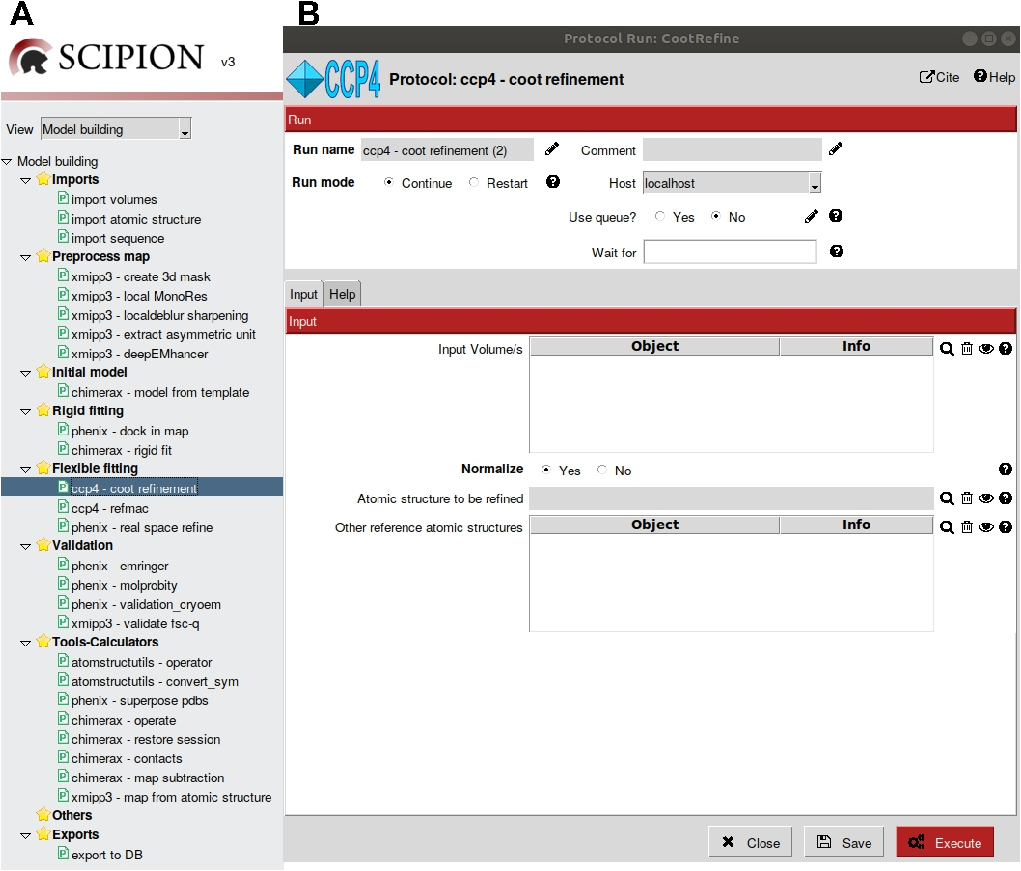
\includegraphics[width=0.90\textwidth]{Images_appendix/Fig119.pdf}
     \caption{Protocol \scommand{ccp4 - coot refinement}. A: Protocol location in \scipion menu. B: Protocol form.}
     \label{fig:app_protocol_coot_1}
    \end{figure}
    
    \begin{itemize}
     \item \ttt{Input} section\\

    \begin{itemize}
     \item \ttt{Input Volume/s}: One or several electron density maps previously downloaded or generated in \scipion. The density volume regarding to which an atomic structure has to be modeled has to be included in this volume list.\\
     \item \ttt{Normalize}: Parameter set to ``Yes'' by default to perform normalization of map electron density levels according to $Coot$ requirements ([0, 1]). This normalization approximates cryo-EM density data to maps obtained from X-ray crystallography because it diminishes Z-score (number of standard deviations) variation of map values.\\  
     \item \ttt{PDB to be refined}: Atomic structure previously downloaded or generated in \scipion. This structure will be fitted and refined according to a particular density volume.\\
     \item \ttt{Other reference PDBs}: Additional atomic structures previously downloaded or generated in \scipion that may be helpful in the refinement process.\\
    \end{itemize}
    \item \ttt{Help} section\\
    This section contains $Coot$ commands to make easier some interactive refinement steps and to save refined atomic structures. Their reference volumes will be saved by default with the refined atomic structures. Here you are an overview of these commands:\\
    \begin{itemize}
     \item Initializing global variables:\\
     Press \ttt{``U''} in your keyboard.\\ 
     \item Automatically moving from one to another chain in an atomic structure:\\
     \begin{itemize}
      \item Press \ttt{``x''} in the keyboard to move from one chain to the previous one.\\
      \item Press \ttt{``X''} to change from one chain to the next one.\\
     \end{itemize} 
     \item Semi-automatic refinement of small groups of residues (10 to 15):\\As soon as $Coot$ protocol is executed, the text file \ttt{coot.ini} will be saved in the project folder \ttt{/Runs/00XXXX\_CootRefine/extra/}. This file content has to be modified according to our atomic structure model in this way:\\
     \begin{itemize}
      \item \ttt{imol: 0}: \#0 has to be replaced by the number of the molecule that has to be refined. This number appears detailed in $Coot$ main menu \ttt{Display Manager} (\ffigure{fig:app_protocol_coot_2} (B, red arrow)).
      \item \ttt{aa\_main\_chain: A}: A has to be replaced by the name of the molecule chain that has to be refined.\\
      \item \ttt{aa\_auxiliary\_chain: AA}: AA, name of the small chain of 10-15 residues, can be optionally replaced by other name.\\
      \item \ttt{aaNumber: 100}: \#100 has to be replaced by the position of the residue from which the refinement has to start.\\
      \item \ttt{step: 10}: \#10 will be replaced by the desired small step of residues that gets flexible enough to select other conformation of this auxiliary chain.\\ 
     \end{itemize} 
     Save \ttt{coot.ini} text file after its modification. Go to the the residue position indicated in \ttt{aaNumber:}, initialize global variables with \ttt{``U''}, and pres \ttt{``z''} in the keyboard
     \item Saving an atomic structure after an interactive working session with $Coot$:\\
     \ttt{Coot Python Scripting} window will be opened with $Coot$ main menu \ttt{Calculate -> Scripting... -> Python...} (\ffigure{fig:app_protocol_coot_2} (A)). By writing \ttt{scipion\_write()} molecule \#0 will be saved by default in \scipion. Molecule number can be checked in $Coot$ main menu \ttt{Display Manager} (\ffigure{fig:app_protocol_coot_2} (B, red arrow)). Saving the molecule this way is equivalent to press \ttt{``w''} in the keyboard.\\The number \# of the specific molecule has to be written in brackets to save any other molecule than \#0.\\Although the name of the saved atomic structure is \ttt{cootOut0001.pdb} by default, other names/labels of your preference are also allowed. That name/label has to be introduced with \ttt{scipion\_write()} command, as it is detailed in the example (\ffigure{fig:app_protocol_coot_2} (A)). The addition of \ttt{.pdb} extension is not required.\\If no more interactive session with $Coot$ are planned, after saving the atomic structure, $Coot$ not will be interactive anymore by pressing \ttt{``e''} in the keyboard.\\
     
      \begin{figure}[H]
       \centering 
       \captionsetup{width=.7\linewidth} 
       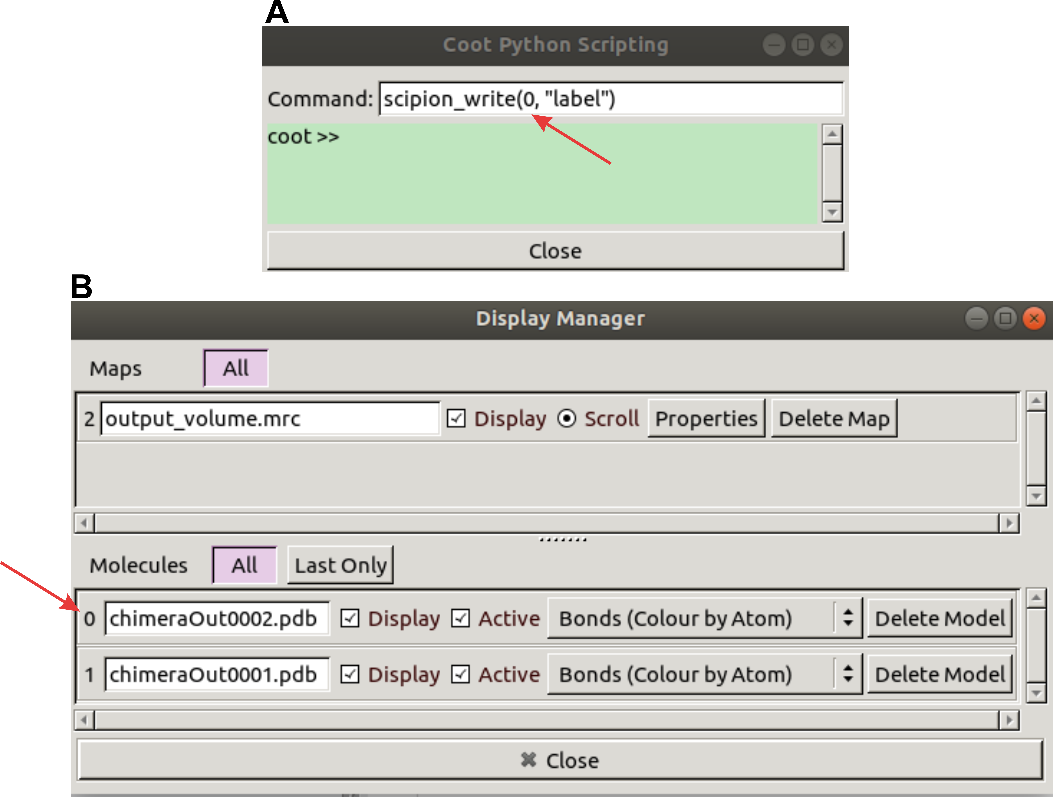
\includegraphics[width=0.80\textwidth]{Images_appendix/Fig120.pdf}
       \caption{Protocol \scommand{ccp4 - coot refinement}. Saving labeled atomic structure with \ttt{Coot Python Scripting} window.}
      \label{fig:app_protocol_coot_2}
     \end{figure}
     
    
     
    \end{itemize}

    
    \end{itemize}
    
\end{itemize}


